\documentclass[a4paper]{article} % A4 paper and 11pt font size

\usepackage{braket}
\usepackage{amsmath}
\usepackage{amssymb}
\usepackage{bm}
\usepackage[utf8]{inputenc}
\usepackage{verbatim}
\usepackage{tikz}
\usepackage{pgfplots}
\usepackage{siunitx}
%\usepackage{pgfornament}
\usepackage{hyperref}
\usepackage{fancyhdr}
\usepackage{pdflscape}
\usepackage{bm}
\usepackage{enumitem}
\usepackage[a4paper]{geometry}
\usepackage{framed}
\usepackage{gensymb}
\usepackage{mathtools} %for underbraces without whitespace (\mathclap{})


\newcommand{\ms}[1]{\SI{#1}{M_{\odot}}}

%for side-by-side figures
\usepackage{graphicx}
\usepackage{caption}
\usepackage{subcaption}


\setlength{\parindent}{2em}
\setlength{\parskip}{1em}
\renewcommand{\baselinestretch}{1.2}

% include this to remove the "References" heading in bibliography
\usepackage{etoolbox}
\patchcmd{\thebibliography}{\section*{\refname}}{}{}{}



\newgeometry{bottom=4cm}

\begin{comment}
 \geometry{
 a4paper,
 total={210mm,297mm},
 left=40mm,
 right=40mm,
 top=20mm,
 bottom=20mm,
 }
 \end{comment}

%----------------------------------------------------------------------------------------
%	TITLE SECTION
%----------------------------------------------------------------------------------------
\setlength\parindent{0pt} % Removes all indentation from paragraphs - comment this line for an assignment with lots of text


\pagenumbering{arabic}
\begin{document}
\pagestyle{empty}

\newcommand{\HRule}{\rule{\linewidth}{0.5mm}}

\begin{titlepage}

    \begin{center}
        \textsc{}\\[3cm]

        \HRule \\[0.5cm]
        %\pgfornament[width = 0.9\textwidth, symmetry=v]{88}\\[0.75cm]        
        \Huge \textbf{PHYC30019 Astrophysics}\\[0.5cm]
        \huge \textbf{Project 3:} ???\\[0.5cm] 
        %\pgfornament[width = 0.9\linewidth]{88}\\[1.5cm]
        \HRule \\[1.5cm]

        \begin{minipage}{0.5\textwidth}
        \begin{center}

		\vspace{3cm}
        \large By \\[0.75cm]
        \begin{tabular}{rl}
        \Large Tyler & \Large \textsc{Gardiner} \\ [0.1cm]
        \Large Braden &\Large \textsc{Moore} \\
		\end{tabular}  
		\\[1cm]
        \normalsize \normalfont 
        The University of Melbourne \\[2cm]

        \end{center}
        \end{minipage}

        \vfill

        \large \today
    \end{center}

\newpage
\end{titlepage}
%----------------------------------------------------------------------------------------
\begin{comment}
\pagestyle{fancy}
\pagenumbering{gobble}
\tableofcontents
\newpage
\end{comment}
\pagenumbering{arabic}
\rfoot{\textsc{PHYC30012 Astrophysics}}

\pagestyle{fancy}
\setcounter{page}{1}
\section*{Motivation}
\begin{framed}
During this workshop you will gain a clearer idea of how the expansion of the universe and its geometry affect the observation of very distant objects. In particular, we want to end by thinking about the sort of experiments you could perform to determine the type of expansion the universe is undergoing. In this workshop, assume that the current values of the energy densities are:
\begin{equation*}
\Omega_{r,0}=10^{-4},\quad \Omega_{m,0}=0.27,\quad \Omega_{\Lambda,0}=0.73
\end{equation*}
You should use an $H_0=\SI{70}{km/sec/Mpc}$. For the order-of-magnitude problems this workshop, try to get to a solution with minimal effort - remember it is an order of magnitude solution you are looking for.
\end{framed}


\section{Order-of-magnitude estimates}
\subsection{Order-of-magnitude estimate 1}
\begin{framed}
Suppose that you have been asked to find new extra-solar planets. You need to think about the techniques that you will use for these experiments. What accuracy is required to detect extra-solar planets by their astrometric wobble? By Doppler shift? Which would you expect to be easier to measure?
\end{framed}

We assume that the plane of the exoplanet's orbit around the observed star is perpendicular to our line-of sight.

As shown in Figure \ref{wobble fig} above, we take the line-of-sight distance from Earth to a star as $d$, and we assume the astronometric wobble of the star due to the exoplanet is
\begin{equation}
r=R_{\text{star}},
\end{equation}
that is, the star's radius.

For small angles we can approximate $\tan\theta\approx \theta$, so that we have
\begin{align}
\tan\theta\approx \theta &= \frac{r}{d}
\intertext{Taking the distance to the star as}
d&\approx \SI{20}{ly}\sim \SI{10}{ly}
\intertext{and the radius as}
r&=M_{\odot}\\
&\approx \SI{7.36d-8}{ly}\\
&\sim \SI{d-7}{ly}
\intertext{we can calculate $\theta$ as}
\theta &= \frac{\SI{d-7}{ly}}{\SI{10}{ly}}\\
&=\SI{d-8}{radians}\\
&=\SI{d-2}{arcsec}
\end{align}
(INCLUDE SOURCES)

That is, we need an angular resolution of $\SI{d-2}{arcsec}$ to detect extra-solar planets by their astronometric wobble. The Hubble Space Telescope has an angular resolution of $\SI{0.05}{arcsec}=\SI{5d-2}{arcsec}$, which we will use as a basis for our ``most accurate'' measurement
\footnote{\url{http://hubblesite.org/hubble_discoveries/hstexhibit/telescope/about.shtml}}. We see that it would be quite difficult to measure this astronometric wobble!

Now we shall investigate the Doppler shift due to wobble.



\subsection{Order-of-magnitude estimate 2}
\begin{framed}
Many galaxies rotate. Can you actually observe the rotation of nearby galaxies over a reasonable (i.e. measureable) timescale?
\end{framed}

We take the average speed of the Solar System to be $\SI{230}{km/s}\sim \SI{200}{km/s}$.

Radius of galaxy $= \SI{7.7}{kpc}\sim \SI{10}{kpc}\sim \SI{3d17}{km}$.

\begin{align}
\text{Distance to thing}&=\frac{\SI{200}{km}}{5}+\SI{50}{yr}\times\frac{\SI{3d7}{s}}{\text{yr}}\\
&=10000\times 3\times 10^7\\
&=3\times 10^{11}\\
&\sim \SI{d11}{km}
\end{align}

\subsection{Order-of-magnitude estimate 3}
\begin{framed}
Consider a galaxy acting as a gravitational lens. You know that the galaxy comprises, stars, globular clusters, dark matter, gas etc. Estimate the probability that a background quasar is gravitationally lensed by a globular cluster, as a function of the probability that is it lensed by the whole galaxy. Can you make a similar estimate for the probability of lensing by a star?

Make sure that you provide details of the criteria that you are using.
\end{framed}

We start by assuming that the relation between $\mathcal{P}_{\text{cluster}}$ and $\mathcal{P}_{\text{galaxy}}$ (where $\mathcal{P}$ is the probability of lensing a background quasar) as
\begin{equation}
\frac{\mathcal{P}_{\text{cluster}}}{\mathcal{P}_{\text{galaxy}}}=\frac{\sigma_{\text{cluster}}}{\sigma_{\text{galaxy}}} \label{probs}
\end{equation}

In equation~(\ref{probs}), $\sigma$ is the cross-sectional area of the object denoted by the subscript. The cross-section $\sigma$ is proportional to $r^2$; instead of the physical radius we will instead use the Einstein radius
\begin{equation}
r \equiv \theta_{\text{ER}} \sim 2''  \left(\frac{M}{10^{12}~M_{\odot}}\right)^{1/2}\left(\frac{D}{\SI{0.3}{Gpc}}\right)^{-1/2}
\end{equation}

This radius takes the galaxy and globular clusters as point-masses, and considers the effect of mass on lensing (which is more important than physically cross-section).

So, we find
\begin{align}
\frac{\mathcal{P}_{\text{cluster}}}{\mathcal{P}_{\text{galaxy}}}
&=\frac{(M_{\text{cluster}}^{1/2})^2}{(M_{\text{galaxy}}^{1/2})^2}\\
&=\frac{M_{\text{cluster}}}{M_{\text{galaxy}}}\\
&=\frac{10^6~M_{\odot}}{10^{12}~M_{\odot}}\\
&=10^{-6}
\end{align}

We use
\begin{align}
M_{\text{cluster}}&=10^6~M_{\odot}\\
M_{\text{galaxy}}&=M_{\text{Milky Way}}=10^{12}~M_{\odot}
\end{align}
SOURCES.

This is actually comparable to using the physical radii,
\begin{align}
\frac{\mathcal{P}_{\text{cluster}}}{\mathcal{P}_{\text{galaxy}}}
&=\frac{r^2_{\text{cluster}}}{r^2_{\text{galaxy}}}\\
&=\frac{0.05^2}{30^2}\\
&=3\times 10^{-6}
\end{align}
SOURCES.



\section{Research Tasks}
\subsection{Research Task 1}
\begin{framed}
When we consider the fluctuations in the CMB, we usually plot a power spectrum to describe the scales where there is most power. Describe the physical quantities that are measured on the two axes of the typical plot of the fluctuations – a full explanation is expected. Then describe the physical interpretation of the two main peaks in the plots.
\end{framed}

The $x$-axis of the plot of fluctuations is masured in multipole moments. The multiploe moment is inversely proportional to the angular scale, meaning that as the multiple moment increases, the angular scale decreases. The angular sclae simply referts to the size of the angle on the sky. The $y$-axis of the CMB power spectrum measures the fluctuation in temperature for a specific angular scale. The fluctation in temperature ($\Delta T$) is measured in microKelvin ($\mu K$).

The first peak in the CMB power spectrum is due to the compression of a large region that reaches its maximum compression at the time of decoupling (STUART'S NOTE). It also shows the size of hot and cold spots ue to this. The most important feature, the angular location of the peak peak, is the geometry of the universe, which is indictated to be spatially flat.

The ratio of the second peak amplitude to the first peak amplitude tells us about the ration of baryon density to the critial density for baryons ($\Omega_b$) \textbf{this is actually baryon energy density, not critical density}.

SOURCES:
\url{background.uchicago.edu/~whu/intermediate/summary.html}

\url{www.astro.umd.edu/~miller/teaching/astr422/lecture21.pdf}


\section{Calculations}

\subsection{Calculation 1}
\begin{framed}
Using the final form of the differential equation that describes the behaviour of the scale factor with time, work out the redshift when dark energy first dominated the expansion of the universe. The equation is given by:
\begin{equation*}
\frac{H^2}{H_0^2}=\frac{\Omega_{r,0}}{R^4}+\frac{\Omega_{m,0}}{R^3}
+\Omega_{\Lambda,0}+\frac{1-\Omega_{0}}{R^2}
\end{equation*}
where the subscript $0$ refers to the present
value and the subscripts $r$, $m$ and $\Lambda$ refer to radiation, matter and the cosmological constant respectively.
\end{framed}

We recall that the Hubble constant $H$ is related to the scale factor $R(t)$ as
\begin{equation}
\frac{\dot{R(t)}}{R(t)}
\end{equation}
where the dot represents a derivative with respect to time. So, we can write the Friedman equation in terms of $R$ by
\begin{align}
\frac{H^2}{H_0^2}&=\frac{\Omega_{r,0}}{R^4}+\frac{\Omega_{m,0}}{R^3}
+\Omega_{\Lambda,0}+\frac{1-\Omega_{0}}{R^2}\\
\Rightarrow \dot{R}^2&=H_0^2 a^2 \left[\frac{\Omega_{r,0}}{R^4}+\frac{\Omega_{m,0}}{R^3}
+\Omega_{\Lambda,0}+\frac{1-\Omega_{0}}{R^2}\right]\\
\Rightarrow \dot{R}&= H_0\left[\frac{\Omega_{r,0}}{R^2}+\frac{\Omega_{m,0}}{R}+\Omega_{\Lambda,0}R^2 + (1-\Omega_0)\right]^{1/2}\label{dot a}
\end{align}

We will assume that the universe is flat;
\begin{equation}
\Rightarrow \Omega_0 = 1
\end{equation}
This is justifiable since $\Omega_0 = \Omega_{r,0}+\Omega_{m,0}+\Omega_{\Lambda,0}\approx 1$ from the values given for this assignment.

Substituting in the energy densities into~(\ref{dot a}) we see
\begin{equation}
\dot{R}= H_0\left[\frac{10^{-4}}{R^2}+\frac{0.27}{R}+0.73R^2\right]^{1/2}
\end{equation}

From this, we can determine when dark energy begins to dominate the expansion of the universe. The era before dark energy-domination is the matter-dominated period. In this period, the effects of radiation on the expansion of the universe are negligible. The redshift at which dark energy and matter both contribute equally to the expansion of the universe is given by
\begin{align}
\Omega_{\Lambda,0}R^2&=\frac{\Omega_{m,0}}{R}\\
\Rightarrow 0.73R^2&=\frac{0.27}{R}\\
\Rightarrow R&=0.718
\intertext{We can write the redshift $z$ in terms of the scale factor as}
\frac{1}{1+z}&=a\\
\Rightarrow z&=\frac{1}{a}-1
\Rightarrow z_{\text{matter-dark energy equality}}&=0.393\label{dm dom}
\end{align}

For all smaller redshifts, dark energy should be the dominant factor in the expansion of the universe (though not exactly, since we have neglected the radiation component, even though it is very small). 

Taking the end of the matter-dominated era as $\SI{9.8d9}{yr}$\footnote{Ryden, Barbara, ``Introduction to Cosmology'', 2006, eqn. 6.33}, we can compare redshifts to see whether out answer is feasible.

In the dark matter-dominated era,
\begin{align}
R&\propto e^{H_0 t}
\intertext{Today we has $R=1$ and $t=t_0$; recalling $t_0=\frac{1}{H_0}$ we have}
1&=Ae^{H_0 t_0}=Ae\\
\Rightarrow A&=e^{-1}\\
\Rightarrow R_{text{matter-dark matter equality}}&=e^{H_0 t - 1}
&=e^{\frac{9.8}{13.8}-1}=0.74
\intertext{Where we have converted $H_0=\SI{70}{km/sec/Mpc}$ into units of $yr$,}
\Rightarrow z_{\text{matter-dark energy equality}}&=\frac{1}{0.74}-1\\
&=0.35
\end{align}

This is indeed close to the redshift we found in~(\ref{dm dom}), so we can justify our approximate value of $z$ calculated early to being around the redshift of the beginning of the dark energy-dominated era.	


\subsection{Calculation 2}
\begin{framed}
For the cosmology given above, use the calculator from the previous workshop to determine the redshift where a galaxy of a standard size has the smallest angular extent or size.

\url{http://www.ph.unimelb.edu.au/cosmocalc/session.php}
\end{framed}

SOURCE: \url{https://ned.ipac.caltech.edu/level5/March02/Sahni/Sahni4_5.html}

Angular size is given by
\begin{equation}
\Delta \theta = \frac{D(1+z)^2}{d_L(z)}
\end{equation}
where $D$ is the proper length of an object, and $d_L$ is the luminosity distance. The proper distance is constant over all redshifts. Using the calculator provided and using the given cosmology, we run over redshift $0.05 \to 5$ in intervals of $0.05$ and use the data to determine the minimum angular size.

A minimum in angular size occurs at $z=0.75$. In Figure \ref{fig:angular size} below we have plotted angular size against distance over our range of values (up to $\sim 3.75$, for illustrative purposes). We see that after reaching the minimum, angular size continues to increase.

\begin{figure}[h]
\centering
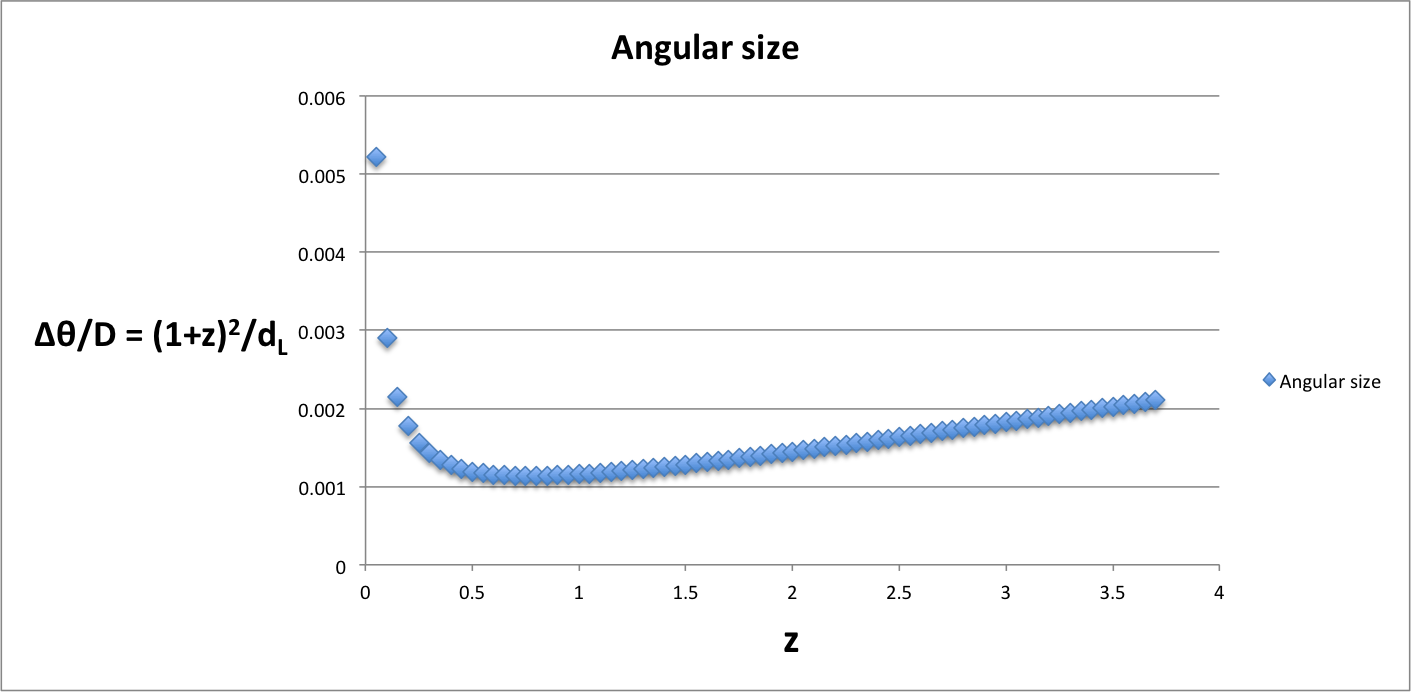
\includegraphics[width=\textwidth]{images/angular-size.png}
\caption{Angular size}
\label{fig:angular size}
\end{figure}


\subsection{Calculation 3}
\begin{framed}
Consider the surface brightness of a galaxy. How is it defined? Now explain how surface brightness changes as a function of distance in a Euclidean, nonexpanding universe. How does surface brightness change in an expanding FRW universe?

What conclusions can you draw about the observations of very distant galaxies?
\end{framed}

The surface brightness is the measured brightness for a specific area on an extended object (e.g. a galaxy). In a Eucllddiean, non-expanindg universe, surface brightness is constant with distance. As distance increases and the brightness fades, the area begin observed also decreases at the same rate.

Flux decreases with the square of the distance, but so does area. So, these values cancel out and the surface brightness is not affected. However, flux is reduced by 2 factors of $(1+z)$, one factor due to time dilation in the photon arrival time, and the other factor for redshift.

\begin{align}
\text{Surface brightness}\equiv\text{SB}&\propto m\\
m & \propto -\log_{10}(\text{flux})\\
\Rightarrow \Delta\text{SB}&\propto -\log_{10}\left(\frac{1}{(1+z)^2}\right)
\end{align}

This suggests that as redshift increases (object is further away), surface brightness decreases. Therefore distant galaxies are axctually brighter than we observe.

\begin{align}
\text{SB}&=m+ 2.5\log_{10}(A)
\intertext{from Wikipedia.}
m&=-2.5\log_{10}\left(\frac{f}{f_0}\right)\\
\text{where } f&=\text{flux},\\
f_0&=\text{reference flux}
\end{align}

\HRule

In a Euclidean, non-expanding universe,
\begin{align}
\text{Surface brightness}\equiv \text{SB}&=m+2.5\log_{10}(A)\\
m&=-2.5\log_{10}(f_E)
\end{align}
where $f_E=\frac{\text{flux}}{\text{relative flux}}$. In an expanding universe,
\begin{align}
f&=\frac{f_E}{(1+z)^2}
\intertext{from lecture notes. Hence,}
\text{SB}&=-2.5\log_{10}\left(\frac{f_E}{(1+z)^2}\right)+2.5\log_{10}(A)\\
&=\underbrace{\left[-2.5\log_{10}(f_E)+2.5\log_{10}(A)\right]}_{\mathclap{\text{independent of distance}}}
+2.5\log_{10}\left(\frac{1}{(1+z)^2}\right)\\
\Rightarrow \Delta \text{SB}&=2.5\log_{10}\left(\frac{1}{(1+z)^2}\right)\\
&=2.5\log_{10}(R^2)\\
&=5\log_{10}R
\end{align}



\section{Conclusion}
\begin{framed}
You have considered some of the changes in observables in different FRW cosmologies. Which observations do you think might be easiest to undertake to measure the curvature of the universe accurately?
\end{framed}

\url{http://map.gsfc.nasa.gov/mission/sgoals_parameters_geom.html}



\pagebreak

\section{References}

\bibliographystyle{plain}
\bibliography{refs.bib}


\end{document}



























